\section{Conceptual Models}

\begin{figure}
\centering
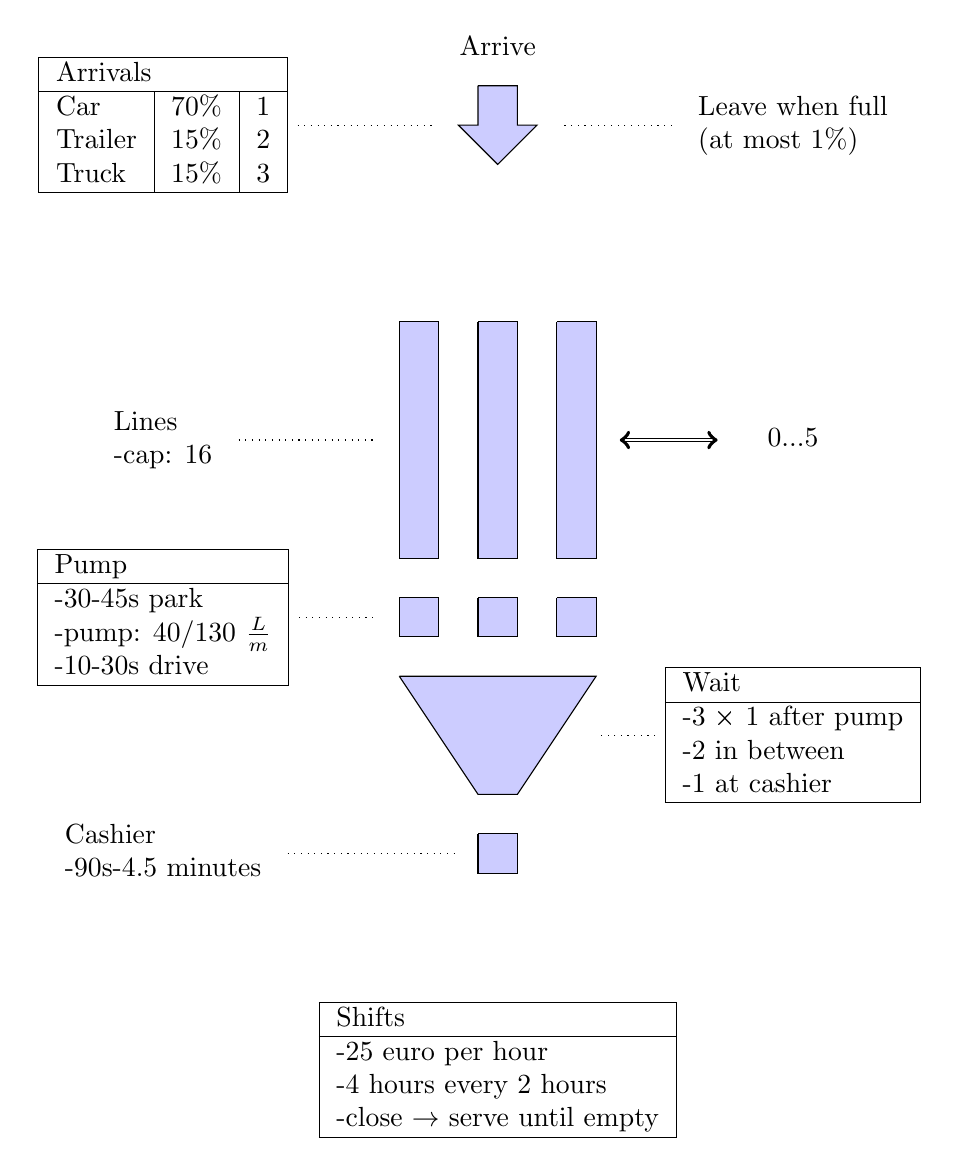
\begin{tikzpicture}

\path[shape=coordinate]
(5,20) coordinate(a11) (5,19.5) coordinate(a12)
(4.75,19.5) coordinate(a13) (5.25,19) coordinate(a14)
(5.75,19.5) coordinate(a15) (5.5,19.5) coordinate(a16)
(5.5,20) coordinate(a17);
\filldraw[fill=blue!20] (a11) -- (a12) -- (a13) -- (a14) -- (a15) -- (a16) -- (a17) -- (a11);

\path[shape=coordinate]
(4,17) coordinate(r11) (4,14) coordinate(r12)
(4.5,14) coordinate(r13) (4.5,17) coordinate(r14);
\filldraw[fill=blue!20] (r11) -- (r12) -- (r13) -- (r14) -- (r11);

\path[shape=coordinate]
(5,17) coordinate(r21) (5,14) coordinate(r22)
(5.5,14) coordinate(r23) (5.5,17) coordinate(r24);
\filldraw[fill=blue!20] (r21) -- (r22) -- (r23) -- (r24) -- (r21);

\path[shape=coordinate]
(6,17) coordinate(r31) (6,14) coordinate(r32)
(6.5,14) coordinate(r33) (6.5,17) coordinate(r34);
\filldraw[fill=blue!20] (r31) -- (r32) -- (r33) -- (r34) -- (r31);

\path[shape=coordinate]
(4,13.5) coordinate(p11) (4,13) coordinate(p12)
(4.5,13) coordinate(p13) (4.5,13.5) coordinate(p14);
\filldraw[fill=blue!20] (p11) -- (p12) -- (p13) -- (p14) -- (p11);

\path[shape=coordinate]
(5,13.5) coordinate(p21) (5,13) coordinate(p22)
(5.5,13) coordinate(p23) (5.5,13.5) coordinate(p24);
\filldraw[fill=blue!20] (p21) -- (p22) -- (p23) -- (p24) -- (p21);

\path[shape=coordinate]
(6,13.5) coordinate(p31) (6,13) coordinate(p32)
(6.5,13) coordinate(p33) (6.5,13.5) coordinate(p34);
\filldraw[fill=blue!20] (p31) -- (p32) -- (p33) -- (p34) -- (p31);

\path[shape=coordinate]
(4,12.5) coordinate(r41) (5,11) coordinate(r42)
(5.5,11) coordinate(r43) (6.5,12.5) coordinate(r44);
\filldraw[fill=blue!20] (r41) -- (r42) -- (r43) -- (r44) -- (r41);

\path[shape=coordinate]
(5,10.5) coordinate(r51) (5,10) coordinate(r52)
(5.5,10) coordinate(r53) (5.5,10.5) coordinate(r54);
\filldraw[fill=blue!20] (r51) -- (r52) -- (r53) -- (r54) -- (r51);

\node[draw=none] at (5.25,20.5) (arr) {Arrive};
\node[draw=none](t1) at (1,19.5){
\begin{tabular}{|l|l|l|}
\hline
\multicolumn{3}{|l|}{Arrivals} \\
\hline
Car     & 70\%  & 1 \\
Trailer & 15\%  & 2 \\
Truck   & 15\%  & 3 \\
\hline
\end{tabular}};
\node[draw=none](t2) at (9,19.5){
\begin{tabular}{l}
Leave when full \\
(at most 1\%)
\end{tabular}};
\node[draw=none](t3) at (1,15.5){
\begin{tabular}{l}
Lines \\
-cap: 16
\end{tabular}};
\node[draw=none](t4) at (1,13.25){
\begin{tabular}{|l|}
\hline
Pump \\
\hline
-30-45s park \\
-pump: 40/130 $\frac{L}{m}$ \\
-10-30s drive \\
\hline
\end{tabular}};
\node[draw=none](t5) at (9,11.75){
\begin{tabular}{|l|}
\hline
Wait \\
\hline
-3 × 1 after pump \\
-2 in between \\
-1 at cashier \\
\hline
\end{tabular}};
\node[draw=none](t6) at (1,10.25){
\begin{tabular}{l}
Cashier \\
-90s-4.5 minutes
\end{tabular}};
\node[draw=none](t7) at (5.25,7.5){
\begin{tabular}{|l|}
\hline
Shifts \\
\hline
-25 euro per hour \\
-4 hours every 2 hours \\
-close $\rightarrow$ serve until empty\\
\hline
\end{tabular}};
\node[draw=none](k9) at (9,15.5){
\begin{tabular}{l}
0...5
\end{tabular}};

\draw[dotted, shorten >= .3cm] (t1) -- (a13);
\draw[dotted, shorten >= .3cm] (t2) -- (a15);
\draw[dotted, shorten >= .3cm] (t3) -- (t3 -| r11);
\draw[dotted, shorten >= .3cm] (t4) -- (t4 -| p11);
\draw[dotted] (t5) -- (t5 -| r44);
\draw[dotted, shorten >= .3cm] (t6) -- (t6 -| r51);

\draw[<->,double, shorten >= .3cm, shorten <= .3cm] (k9) -- (k9 -| r34);

\end{tikzpicture}
\caption{Conceptual model Nicky Advokaat}
\end{figure}

\textbf{Problems of the model}
\begin{enumerate}
\item There is no clear flow between the states.
\item The number of queues is incorrect.
\item The action cleans windows is missing from the pump actions.
\end{enumerate}

\newpage

\begin{figure}
\centering
\begin{tikzpicture}[
place/.style={
rectangle,
minimum size=6mm,
semithick,
draw=black,
fill=blue!20
},
title/.style={
draw=none,
fill=none,
color=gray,
anchor=west
},
ptext/.style={
draw=none,
fill=none,
color=black
},
superplace/.style={
matrix of nodes,
nodes=place,
row 1/.style={
    nodes=title
},
row sep=0.5em,
column sep={3em,between origins},
matrix anchor=north,
rectangle,
semithick,
draw=black,
fill=orange!20
}]

\matrix[row sep = 3em] (mat) {
\node [draw=none] (track) {Trucks}; &
\node [draw=none] (cave) {Cars + trailer}; &
\node [draw=none] (car) {Cars}; &\\

&\node [place] (enter) {Enter station}; & & \\

&\node [place] (choose) {Choose (shortest) lane}; & & \node [draw=none](t1) {
\begin{tabular}{l}
Leave if all \\ lanes blocked
\end{tabular}}; \\
&\node [place] (queue) {Queue}; & & \\
&\node [place] (getf) {Get fuel}; & & \node[draw=none] (t2) {and clean windows}; \\
&\node [place] (queue2) {Queue}; & & \\
&\node [place] (pay) {Pay at cashier}; & & \\
&\node [place] (leave) {Leave}; & & \\
};

\node [draw=none,below =of mat] {This does not include leaving/taking over shifts};

\draw[->,thick] (car) -- (enter.north east);
\draw[->,thick] (cave) -- (enter.north);
\draw[->,thick] (track) -- (enter.north west);

\draw[->,thick] (enter) -- (choose);
\draw[->,thick] (choose) -- (queue);
\draw[->,thick] (queue) -- (getf);
\draw[->,thick] (getf) -- (queue2);
\draw[->,thick] (queue2) -- (pay);
\draw[->,thick] (pay) -- (leave);

\draw[->,thick] (choose) -- (t1);
\draw[->,thick] (t2) -- (getf);

\end{tikzpicture}
\caption{Conceptual model Robbert Jongeling}
\end{figure}

\textbf{Problems of the model}
\begin{enumerate}
\item The arrival percentages are missing.
\item The number of queues are missing.
\item The different actions in the fuel state are missing.
\item Information about the fuel times and waiting times is missing.
\end{enumerate}

\newpage

\begin{figure}
\centering
\begin{tikzpicture}[
place/.style={
rectangle,
minimum size=6mm,
semithick,
draw=black,
fill=blue!20
},
title/.style={
draw=none,
fill=none,
color=gray,
anchor=east
},
ptext/.style={
draw=none,
fill=none,
color=black
},
superplace/.style={
matrix of nodes,
nodes=place,
row 1/.style={
    nodes=title
},
row sep=0.5em,
column sep={3em,between origins},
matrix anchor=north,
rectangle,
semithick,
draw=black,
fill=orange!20
}]

\node [draw=none] (cave) {};
\node [place,below =of cave] (arr) {Arriving};

\matrix [superplace,below of=arr](queueing){
    Queueing & & &\\
    & |(selq)| Select Queue & &\\
    & & &\\
    & & &\\
    & & &\\
    |[label=below:$1$,inner sep=0](q1)|\rotatebox{90}{\tbsep} & |[label=below:$2$,inner sep=0](q2)|\rotatebox{90}{\tbsep} &  & |[label=below:$15$,inner sep=0](q15)|\rotatebox{90}{\tbsep} \\
};

\node [draw=none, left =of queueing] (block) {};

\matrix [superplace,below =of queueing](refueling){
    Refueling\\
    |(park)| Parking\\
    |(ref)| Refueling\\
    |(clean)| Clean windows\\
};

\matrix [superplace,below =of refueling](caque){
    Cashier \\
     |[label=below:$1$,inner sep=0](c1)|\rotatebox{90}{\tbsep} & |[label=below:$2$,inner sep=0](c2)|\rotatebox{90}{\tbsep} &  & |[label=below:$5$,inner sep=0](c5)|\rotatebox{90}{\tbsep} \\
};

\node [place,right =of caque] (pay) {Paying};
\node [draw=none, right =of pay] (lea) {Vehicle leaves};

\node [draw=none] at (7,-0.5) (t1) {
\begin{tabular}{|l | l|}
\hline
\multicolumn{2}{|l|}{Vehicles}\\
\hline
70\% & Car \\ 15\% & Car with trailer \\ 15\% & Truck \\
\hline
\end{tabular}};
\node [draw=none] at (7,-3.8)(t2) {
\begin{tabular}{|l|}
\hline
Vehicles select shortest open queue\\
\hline
At most 1\% blocked\\
\hline
\end{tabular}};
\node [draw=none] at (7,-6)(t3) {
\begin{tabular}{|l|l|}
\hline
\multicolumn{2}{|l|}{Max waiting time} \\
\hline
Car & \multirow{2}{*}{30 min (1800 sec)} \\
(with trailer) & \\
Truck & 45 min (2700 sec) \\
\hline
\end{tabular}};
\node [draw=none] at (5.6,-9.2)(t4) {
\begin{tabular}{|l|}
\hline
30-45 seconds \\
\hline
\end{tabular}};
\node [draw=none] at (7,-10.7)(t5) {
\begin{tabular}{|l|l|}
\hline
\multicolumn{2}{|l|}{Time, depends on fuel amount} \\
\hline
Car & \multirow{2}{*}{fuel / 40 min} \\
(with trailer) & \\
Truck & fuel / 130 min \\
\hline
\end{tabular}};
\node [draw=none] at (5.6,-12.2)(t6) {
\begin{tabular}{|l|}
\hline
10-30 seconds \\
\hline
\end{tabular}};
\node [draw=none] at (7,-14.2)(t7) {
\begin{tabular}{|l|}
\hline
Pick cashier queue corresponding\\
to lane (1-3$\rightarrow$1, 4-6$\rightarrow$2, etc) \\
\hline
\end{tabular}};
\node [draw=none] at (6.5,-17.3)(t8) {
\begin{tabular}{|l|}
\hline
Typically 90 seconds\\
Maximum 4.5 min (270 sec) \\
\hline
\end{tabular}};

\draw[->,thick] (cave) --  coordinate[midway](m)(arr.north);

\draw[->,thick] (arr.south -| selq.north) -- (selq.north);

\draw[->,thick] (selq.west) -- (selq.west -| block) node[midway,below,draw=none] {Blocked};
\draw[->,thick] (pay.east) -- (lea.west);

\draw[->,thick] (selq.south -| q1.north) -| (q1.north);
\draw[->,thick] (selq.south -| q2.north) -- (q2.north);
\draw[->,thick] (selq.east) -| (q15.north);

\draw[->,thick] (queueing.south) -- (refueling.north);
\draw[->,thick] (refueling.south) -- (caque.north);
\draw[->,thick] (caque.east |- pay.west) -- (pay.west);

\draw[dotted, shorten >= .3cm, shorten <= .3cm] (q2) -- (q15);

\draw[dotted,semithick] (t1.west |- m) -- (m);
\draw[dotted,thick,bend right=45] (t2.north west) to (selq.north east);
\draw[dotted,semithick] (t3.west |- q15) -- (q15);

\draw[dotted,thick] (t4.west) -- (park.east);
\draw[dotted,semithick] (t5.west |- ref) -- (ref);
\draw[dotted,semithick] (t6.west |- clean) -- (clean);

\draw[dotted,semithick] (t7.west -| caque.east) -- (t7);
\draw[dotted,semithick] (t8.north -| pay) -- (pay);

\draw[dotted, shorten >= .3cm, shorten <= .3cm] (c2.east) -- (c5.west);

\end{tikzpicture}
\caption{Conceptual model Bram Kohl}
\end{figure}

\textbf{Problems of the model}
\begin{enumerate}
\item There were no clear problems with this model.
\end{enumerate}

\newpage

\begin{figure}
\centering
\begin{tikzpicture}[
place/.style={
rectangle,
minimum size=6mm,
semithick,
draw=black,
fill=blue!20
},
title/.style={
draw=none,
fill=none,
color=gray,
anchor=west
},
ptext/.style={
draw=none,
fill=none,
color=black
},
superplace/.style={
matrix of nodes,
nodes=place,
row 1/.style={
    nodes=title
},
row sep=0.5em,
column sep={3em,between origins},
matrix anchor=north,
rectangle,
semithick,
draw=black,
fill=orange!20
}]
\node [draw=none] (cave) {Car + Vehicle};
\node [draw=none,left =of cave] (car) {Car};
\node [draw=none,right =of cave] (track) {Truck};

\node [place,below =of cave] (arr) {Arriving};

\matrix [superplace,below of=arr](queueing){
    Queueing & & & &\\
    & & |(selq)| Select Queue & &\\
    & & & &\\
    & & & &\\
    & & & &\\
    & |[label=below:$1$,inner sep=0](q1)|\rotatebox{90}{\tbsep} & |[label=below:$2$,inner sep=0](q2)|\rotatebox{90}{\tbsep} &  & |[label=below:$15$,inner sep=0](q15)|\rotatebox{90}{\tbsep} \\
};

\node [place,below =of queueing] (pump) {Pump};
\node [place,below =of pump] (queue) {Queue};
\node [place,below =of queue] (pay) {Pay};
\node [place,below =of pay] (leave) {Leave};

\node [draw=none] at (7,-1.5)(t1) {
\begin{tabular}{l}
70\% Car \\ 15\% Car with trailer \\ 15\% Truck
\end{tabular}};
\node [draw=none] at (7,-3.8)(t2) {Select shortest queue};
\node [draw=none] at (7,-5.5)(t3) {
\begin{tabular}{l}
Staffing costs \\ Cashier 25,- per hour
\end{tabular}};
\node [draw=none, right=2cm of pump](t4) {
\begin{tabular}{l}
Park the car: 30-45 sec \\ Refuels, clean the windows,\\ start again: 10-30s
\end{tabular}};
\node [draw=none, right=2cm of pay](t5) {
\begin{tabular}{l}
Avg transaction time: 90s \\ Max transaction time: 270s
\end{tabular}};

\node [draw=none, below=of leave](t6) {
\begin{tabular}{l l}
Car(with trailer) &avg at most 30 min \\ Truck &avg at most 45 min
\end{tabular}};

\draw[->,thick] (car) -- (arr.north west);
\draw[->,thick] (cave) -- (arr.north);
\draw[->,thick] (track) -- (arr.north east);

\draw[->,thick] (arr.south -| selq.north) -- (selq.north);

\draw[->,thick] (selq.south -| q1.north) -- (q1.north);
\draw[->,thick] (selq.south -| q2.north) -- (q2.north);
\draw[->,thick] (selq.east) -| (q15.north);

\draw[dotted, shorten >= .5cm, shorten <= .5cm] (q2) -- (q15);

\draw[->,thick] (queueing) -- (pump);
\draw[->,thick] (pump) -- (queue);
\draw[->,thick] (queue) -- (pay);
\draw[->,thick] (pay) -- (leave);

\draw[->,thick, shorten >= .5cm] (t1.west |- arr) -- (arr);
\draw[->,thick, shorten >= 2cm] (t2.west |- selq) -- (selq);
\draw[->,thick, shorten >= .5cm] (t3.west |- queueing) -- (queueing);
\draw[->,thick, shorten >= .5cm] (t4) -- (pump);
\draw[->,thick, shorten >= .5cm] (t5) -- (pay);

\end{tikzpicture}
\caption{Conceptual model Jasper Selman}
\end{figure}

\textbf{Problems of the model}
\begin{enumerate}
\item Misses info in the pump state about the refuelling.
\item It is not possible for a car to get blocked and therefore not go into a queue.
\end{enumerate}

\newpage

\begin{figure}
\centering
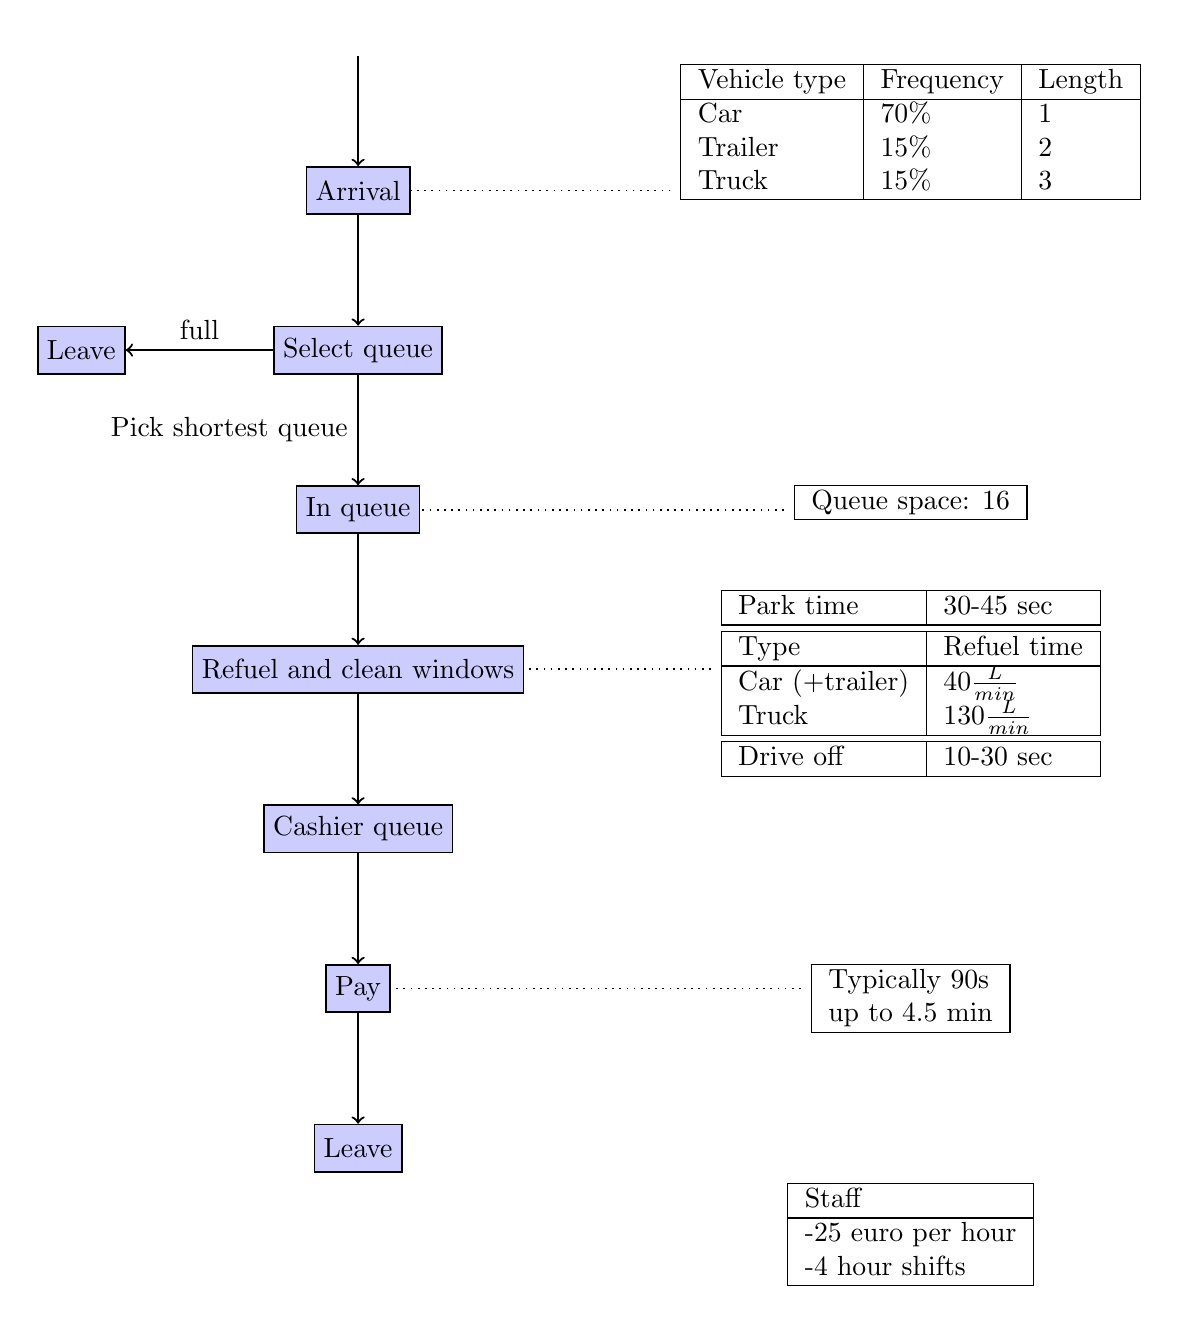
\begin{tikzpicture}[
place/.style={
rectangle,
minimum size=6mm,
semithick,
draw=black,
fill=blue!20
}]

\matrix[row sep=4em,column sep={10em,between origins}]{
                            &   \node[draw=none] (s) {};                \\
                            &   \node[place] (arr) {Arrival};           \\
\node[place] (l1) {Leave};  &   \node[place] (selq) {Select queue};     \\
                            &   \node[place] (queue) {In queue};        \\
                            &   \node[place] (ref) {Refuel and clean windows};            \\
                            &   \node[place] (cash) {Cashier queue};    \\
                            &   \node[place] (pay) {Pay};               \\
                            &   \node[place] (l2) {Leave};              \\
};

\node[draw=none](t1) at (8,6){
\begin{tabular}{|l|l|l|}
\hline
Vehicle type & Frequency & Length\\
\hline
Car     & 70\%  & 1 \\
Trailer & 15\%  & 2 \\
Truck   & 15\%  & 3 \\
\hline
\end{tabular}};
\node[draw=none](t2) at (8,1.3){
\begin{tabular}{|l|}
\hline
Queue space: 16 \\
\hline
\end{tabular}};
\node [draw=none] at (8,-1)(t3) {
\begin{tabular}{|l|l|}
\hline
Park time & 30-45 sec \\
\hline
\hline
Type & Refuel time \\
\hline
Car (+trailer) & $40 \frac{L}{min}$ \\
Truck & $130 \frac{L}{min}$ \\
\hline
\hline
Drive off & 10-30 sec \\
\hline
\end{tabular}};
\node[draw=none](t4) at (8,-5){
\begin{tabular}{|l|}
\hline
Typically 90s \\
up to 4.5 min \\
\hline
\end{tabular}};
\node[draw=none](t5) at (8,-8){
\begin{tabular}{|l|}
\hline
Staff \\
\hline
-25 euro per hour \\
-4 hour shifts \\
\hline
\end{tabular}};

\draw[->,thick] (s) -- (arr);
\draw[->,thick] (arr) -- (selq);
\draw[->,thick] (selq) -- (l1) node[draw=none,midway,above]{full};
\draw[->,thick] (selq) -- (queue) node[draw=none,midway,left]{Pick shortest queue};
\draw[->,thick] (queue) -- (ref);
\draw[->,thick] (ref) -- (cash);
\draw[->,thick] (cash) -- (pay);
\draw[->,thick] (pay) -- (l2);

\draw[dotted,semithick] (t1.west |- arr) -- (arr);
\draw[dotted,semithick] (t2.west |- queue) -- (queue);
\draw[dotted,semithick] (t3.west |- ref) -- (ref);
\draw[dotted,semithick] (t4.west |- pay) -- (pay);

\end{tikzpicture}
\caption{Conceptual model Ramon de Vaan}
\end{figure} 

\textbf{Problems of the model}
\begin{enumerate}
\item Misses info about the cashier queue.
\item Misses the percentage of blocked vehicles.
\item Misses the number of queues.
\end{enumerate}